\documentclass[a4paper]{article}
\usepackage[utf8]{inputenc}
\usepackage[english, russian]{babel}
\usepackage{geometry,
            amsmath,
            hyperref,
            graphicx}
\geometry{left=20mm,
        right=10mm,
        top=30mm,
        bottom=20mm}
\graphicspath{ {./images/} }

\begin{document}

    \begin{titlepage}
        \centering
        {\Large\bfseries Правительство Российской Федерации     \\
            ФЕДЕРАЛЬНОЕ ГОСУДАРСТВЕННОЕ АВТОНОМНОЕ \\
            ОБРАЗОВАТЕЛЬНОЕ УЧРЕЖДЕНИЕ ВЫСШЕГО ОБРАЗОВАНИЯ \\
            «НАЦИОНАЛЬНЫЙ ИССЛЕДОВАТЕЛЬСКИЙ УНИВЕРСИТЕТ \\
            «ВЫСШАЯ ШКОЛА ЭКОНОМИКИ» \\
        (НИУ ВШЭ) }

        
        \vspace{1cm}
        
        {\Large Московский институт электроники и математики им. Тихонова Департамент электронной инженерии}
        
        \vspace{2cm}
        
        {\large ОТЧЕТ \\
            О ПРАКТИЧЕСКОЙ РАБОТЕ № 2 \\
            по дисциплине «Математические основы защиты информации» \\
            ТЕМА РАБОТЫ \\
            Матричный шифр Хилла
        }
        
        \vspace{6cm}
        \begin{flushright}
            {\large Выполнил: \\
            Студент группы БИБ202 \\
            Кудайбергенов Амиржан \\
            25.04.2022г.\\
            Руководитель \\
            Заведующий кафедрой информационной \\
            безопасности киберфизических систем \\
            канд. техн. наук, доцент \\
            \verb|______________|О.О. Евсютин \\
            «\verb|___|»\verb|__________| 2022 г. \\ }
        \end{flushright}
        
        \vfill
        
        {\itshape Москва 2022}
    \end{titlepage}

\newpage

\pagenumbering{roman}

\tableofcontents 

\pagebreak

\pagenumbering{arabic}

\section{Цель работы}

Целью данной работы является приобретение навыков программной реализации и криптоанализа применительно к блочному шифру Хилла.

\section{Краткая теоретическая часть}

\subsection{Описание шифров}

Шифр Хилла \\
Данный шифр построен на основе матричных преобразований. \\
Множество невырожденных квадратных матриц над кольцом классов вычетов по модулю n образует группу. \\\
Открытый текст разбивается на блоки длиной n, и каждый блок представляется в виде n-мерного вектора.

\[
    X=Y=(Z_m)^n.
\]

Ключом является квадратная матрица размера n$\times$n.

\[
    K=GL_n(Z_n).
\]

\[
    k=(k_{i,j}),i,j=\overline{1,n},k_{i,j} \in Z_m.
\]

Эта матрица должна быть обратима в $Z_m$, чтобы была возможна операция расшифрования. Матрица будет являться обратимой только в том случае, если ее детерминант не равен нулю и не имеет общих делителей с основанием модуля. 

\[
    |k| \in Z^*_m.
\]

Операция зашифрования заключается в том, что вектор, соответствующий блоку открытого текста, умножается на ключевую матрицу. 

\[
    x=(x_1,...,x_n)^T.
\]

\[
    y=(y_1,...,y_n)^T=E_k(X)=k
    \begin{pmatrix}
        x_1 \\
        \vdots \\
        x_n \\
    \end{pmatrix}
    =
    \begin{pmatrix}
        y_1 \\
        \vdots \\
        y_n \\
    \end{pmatrix}
    .
\]

Для того, чтобы расшифровать шифртекст, необходимо, разбив его на блоки, представить каждый блок в виде вектора и умножить на обратную матрицу ключа.
В случае рекуррентного шифра Хилла для каждого блока открытого текста вычисляется новое ключевое значение на основе двух предыдущих.

\[
    k_{i+1}=k_i k_{i-1}.
\]

\[
    k^{-1}_{i+1}=k^{-1}_{i-1} k^{-1}_i.
\]

\subsection{Методы криптоанализа шифров}

\section{Примеры шифрования}

\subsection{Шифр Хилла}

1. В следующем примере будем использовать латинские буквы от A до Z, соответствующие им численные значения приведены в таблице. Целесообразно добавить к алфавиту еще 3 символа чтобы длина алфавита была простым числом. Потому что для расшифровки необходимо, чтобы детерминант ключа и длина алфавита были взаимно простыми.

2. Теперь берем текст, который хотим зашифровать и кодируем его с помощью нашего алфавита. Возьмем для примера слово “KERNEL” его код: 10 4 17 13 4 11.

3. Теперь выбираем ключевое слово. Например: OPENSTACK. Получаем:

\[
    K=
    \begin{pmatrix}
        14 & 15 & 4 \\
        13 & 18 & 19 \\
        0 & 2 & 10 \\
    \end{pmatrix},
    P_1=
    \begin{pmatrix}
        10 \\
        4 \\
        17 \\
    \end{pmatrix},
    P_2=
    \begin{pmatrix}
        13 \\
        4 \\
        11 \\
    \end{pmatrix}
\]

Данная матрица обратима, так как её детерминант не равен нулю и не имеет общих делителей с основанием модуля.

\[
    C_1=K*P_1 (mod 29)=
    \begin{pmatrix}
        14 & 15 & 4 \\
        13 & 18 & 19 \\
        0 & 2 & 10 \\
    \end{pmatrix}
    \begin{pmatrix}
        10 \\
        4 \\
        17 \\
    \end{pmatrix}
    (mod 29) =
    \begin{pmatrix}
        7 \\
        3 \\
        4 \\
    \end{pmatrix}
    ,
\]

\[
    C_2=K*P_2 (mod 29)=
    \begin{pmatrix}
        14 & 15 & 4 \\
        13 & 18 & 19 \\
        0 & 2 & 10 \\
    \end{pmatrix}
    \begin{pmatrix}
        13 \\
        4 \\
        11 \\
    \end{pmatrix}
    (mod 29) =
    \begin{pmatrix}
        25 \\
        15 \\
        2 \\
    \end{pmatrix}
    .
\]

Получаем шифртекст HDEZPC

4. Расшифрование \\
Обратная матрица ключа: 

\[
    K^{-1} (mod 26)=
    \begin{pmatrix}
        1 & 28 & 16 \\
        24 & 21 & 23 \\
        1 & 19 & 10 \\
    \end{pmatrix}
\]

Возьмём ранее выведенный шифртекст

\[
    P_1=K^{-1}*C_1 (mod 29)=
    \begin{pmatrix}
        1 & 28 & 16 \\
        24 & 21 & 23 \\
        1 & 19 & 10 \\
    \end{pmatrix}
    \begin{pmatrix}
        7 \\
        3 \\
        4 \\
    \end{pmatrix}
    (mod 29) =
    \begin{pmatrix}
        10 \\
        4 \\
        17 \\
    \end{pmatrix}
    ,
\]

\[
    P_2=K^{-1}*C_2 (mod 29)=
    \begin{pmatrix}
        1 & 28 & 16 \\
        24 & 21 & 23 \\
        1 & 19 & 10 \\
    \end{pmatrix}
    \begin{pmatrix}
        25 \\
        15 \\
        2 \\
    \end{pmatrix}
    (mod 29) =
    \begin{pmatrix}
        13 \\
        4 \\
        11 \\
    \end{pmatrix}
    .
\]
   
\subsection{Рекуррентный шифр Хилла}

Главное отличие рекуррентного шифра от простого состоит в том что для каждого блока открытого текста вычисляется новое ключевое значение на основе двух предыдущих. Для примера возьмем слово “TABLES” а первый два ключа: “ARCH”; “LINK”, алфавит также 29 символа.

\[
    k_1=
    \begin{pmatrix}
        0 & 17 \\
        2 & 7
    \end{pmatrix},
    k_2=
    \begin{pmatrix}
        11 & 8 \\
        13 & 10
    \end{pmatrix},
    P_1=
    \begin{pmatrix}
        19 \\
        0
    \end{pmatrix},
    P_2=
    \begin{pmatrix}
        1 \\
        11
    \end{pmatrix},
    P_3=
    \begin{pmatrix}
        4 \\
        18
    \end{pmatrix}
\]

Зашифруем:

\[
    C_1=
    \begin{pmatrix}
        0 & 17 \\
        2 & 7
    \end{pmatrix}
    \begin{pmatrix}
        19 \\
        0
    \end{pmatrix}
    (mod 29) =
    \begin{pmatrix}
        0 \\
        9
    \end{pmatrix}
\]

\[
    C_2=
    \begin{pmatrix}
        11 & 8 \\
        13 & 10
    \end{pmatrix}
    \begin{pmatrix}
        1 \\
        11
    \end{pmatrix}
    (mod 29) =
    \begin{pmatrix}
        12 \\
        7
    \end{pmatrix}
\]

\[
    C_3=
    \begin{pmatrix}
        11 & 8 \\
        13 & 10
    \end{pmatrix}
    \begin{pmatrix}
        0 & 17 \\
        2 & 7
    \end{pmatrix}
    \begin{pmatrix}
        4 \\
        18
    \end{pmatrix}
    (mod 29) =
    \begin{pmatrix}
        16 & 243 \\
        20 & 291
    \end{pmatrix}
    \begin{pmatrix}
        4 \\
        18
    \end{pmatrix}
    (mod 29) =
    \begin{pmatrix}
        1 \\
        11
    \end{pmatrix}
\]

Обратные матрицы ключей: 

\[
    k^{-1}_1=
    \begin{pmatrix}
        16 & 15 \\
        12 & 0
    \end{pmatrix},
    k^{-1}_2=
    \begin{pmatrix}
        21 & 18 \\
        22 & 26
    \end{pmatrix},
    k^{-1}_3=
    \begin{pmatrix}
        666 & 678 \\
        252 & 216
    \end{pmatrix}
\]

Дешифруем:

\[
    P_1=
    \begin{pmatrix}
        16 & 15 \\
        12 & 0
    \end{pmatrix}
    \begin{pmatrix}
        0 \\
        9
    \end{pmatrix}
    (mod 29) =
    \begin{pmatrix}
        19 \\
        0
    \end{pmatrix},
\]

\[
    P_2=
    \begin{pmatrix}
        21 & 18 \\
        22 & 26
    \end{pmatrix},
    \begin{pmatrix}
        12 \\
        7
    \end{pmatrix}
    (mod 29) =
    \begin{pmatrix}
        1 \\
        11
    \end{pmatrix}
\]

\[
    P_3=
    \begin{pmatrix}
        666 & 678 \\
        252 & 216
    \end{pmatrix}
    \begin{pmatrix}
        1 \\
        11
    \end{pmatrix}
    (mod 29) =
    \begin{pmatrix}
        4 \\
        18
    \end{pmatrix}
\]

\section{Программная реализация шифров}
Реализация представляет собой 2 отдельных файла. У каждого шифра есть два
режима работы: либо используется ввод строки с дальнейшим выводом в терминал, либо режим работы с файлом где вывод сохраняется в двух отдельных файлах. В реализации представлены вывод шифртекста и расшифрованный текст по шифртексту. Исходный код можно посмотреть в репозитории \url{https://github.com/kud-aa/mozi_practics}

\begin{figure}[h]
    \centering
    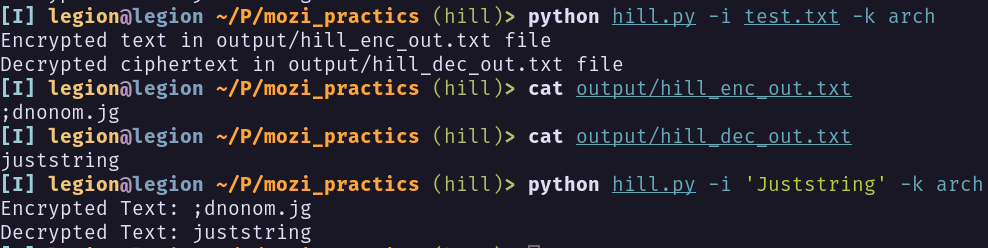
\includegraphics[width=\textwidth]{hill_1.png}
    \caption{Вывод шифра Хилла}
\end{figure}

\begin{figure}[h]
    \centering
    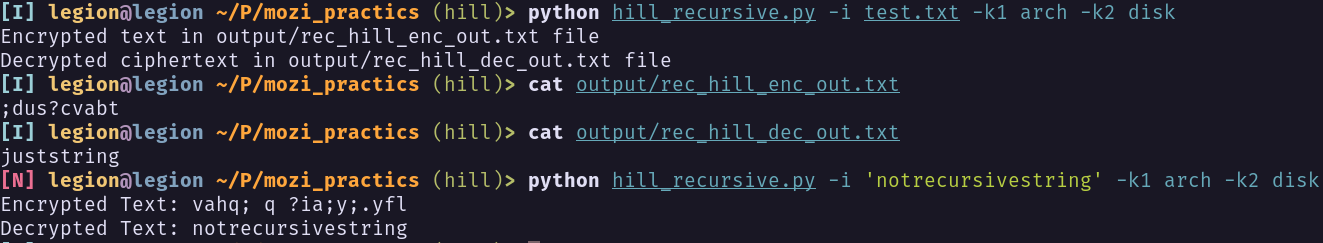
\includegraphics[width=\textwidth]{hill_2.png}
    \caption{Вывод рекуррентного шифра Хилла}
\end{figure}

\section{Примеры криптоанализа}

Стандартный шифр Хилла имеет пространство ключей $n^{m^2}$, где n-мощность алфавита m-мощность ключа или сколько существует матриц размера m на m. Для рекуррентного шифра это число возводиться в квадрат поэтому полный перебор не будет эффективен. 

Также шифр Хилла стоек к частотному анализу так как не будет соответсвия между одинаковыми символами даже для стандартной вариации. 

Поэтому будем использовать атаку по открытому тексту потому что в нём используются линейные операции.

\begin{figure}[h]
    \centering
    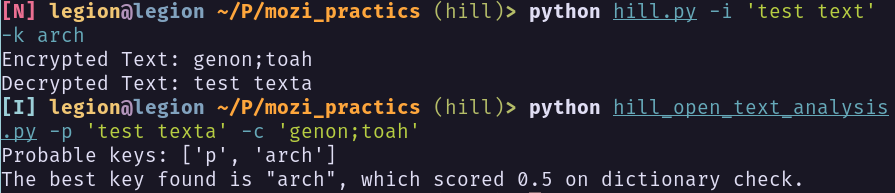
\includegraphics[width=\textwidth]{hill_3.png}
    \caption{Вывод криптоанализа шифра Хилла}
\end{figure}


В отличии от стандартного шифра Хилла для рекуррентной версии требуется минимум m пар текста и шифратекста. 

\begin{figure}[h]
    \centering
    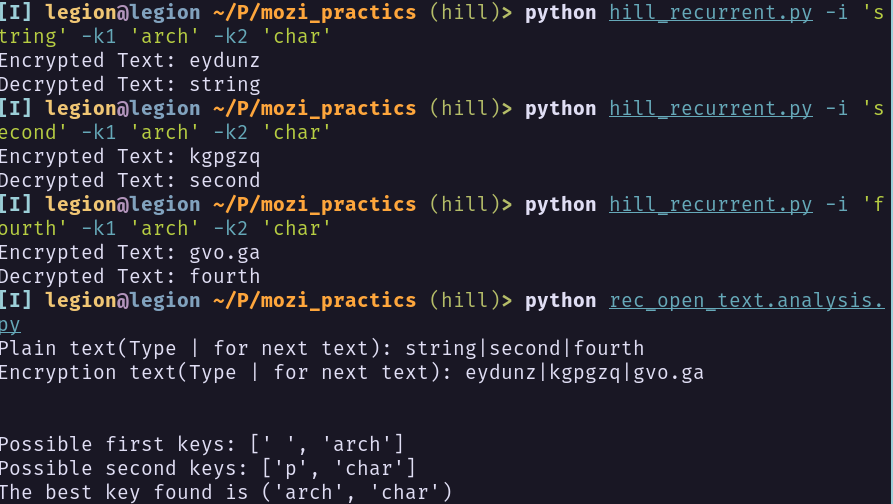
\includegraphics[width=\textwidth]{hill_4.png}
    \caption{Вывод криптоанализа рекуррентного шифра Хилла}
\end{figure}

\section{Выводы о проделанной работе}
В процессе изучения программной реализации и криптоанализа шифра Хилла и его рекуррентной версии. Сделан вывод о их нестойкости (за исключением последнего при условии достаточно большого алфавита) к методам современной криптографии.

\end{document}
